%----------------------------------------------------------------------------------------
%	PACKAGES AND OTHER DOCUMENT CONFIGURATIONS
%----------------------------------------------------------------------------------------
% The file aaai.sty is the style file for AAAI Press 
% proceedings, working notes, and technical reports.
%

\documentclass[letterpaper]{article}
\usepackage{aaai}
\usepackage{times}
\usepackage{helvet}
\usepackage{courier}

\usepackage{graphicx} % support the \includegraphics command and options
\graphicspath{{image/}}

\begin{document}

%----------------------------------------------------------------------------------------
%	TITLE SECTION
%----------------------------------------------------------------------------------------

\title{Understanding YouTube Engagement}
\author{Siqi Wu\\
% Australian National University, Data61 CSIRO\\
}

% Print the title
\maketitle

\begin{abstract}
\begin{quote}
Abstract here...
\end{quote}
\end{abstract}

%----------------------------------------------------------------------------------------
%	ARTICLE CONTENTS
%----------------------------------------------------------------------------------------

\section{Introduction}
\subsubsection{Importance of analysing watch time.} YouTube starts to stress on watch time rather than view number.

\subsubsection{A metric to quantify video quality.} Quality of video is a loose defined concept. We use video watch percentage as a proxy to measure video quality.

\subsubsection{Cold-start predicting watch percentage}

%----------------------------------------------------------------------------------------

\section{Related work}

\subsubsection{YouTube viewing behavior} Video watch time associates with popularity metrics (e.g., view count, the number of comments and shares) and user reaction (e.g., sentiment polarity of comments, the number of likes and dislikes) collectively \cite{Park:2016data}. However, their observations base on a prior observation period, while our foucs is different, without observing an early reaction from video audiences, can we predict watch percentage from a cold start setting up? Or can we classify a bunch of quality videos?

\subsubsection{Model of predicting future view count} Peeking strategy and \textit{ex-ante} prediction \cite{martin2016exploring}.

%----------------------------------------------------------------------------------------

\section{Data and measurement}

\subsection{Data Collection}

\subsubsection{Random Videos.} To obtain a sample of YouTube videos, we used Twitter appearance as a selecting policy. With the help of Twitter Streaming API, first we crawled 202 million tweets that contained "YouTube" keyword over two months period, from July 1st, 2016 to August 30th, 2016. We then parsed the associated shortened URL and only considered tweets that linked to a genuine YouTube video page. Out of these, 36 million video IDs were identified. Finally, we used YouTube Data API and YTCrawl tool \cite{Yu:2015lifecyle} to acquire video metadata and daily viewing statistics respectively. After accounting the effects of Twitter sampling, video attrition and private statistics, our \textit{Random Videos} resulted in a total set of \textit{20} million YouTube videos. Furthermore, we aggregated these random videos by category to constitute \textit{Random Music} dataset, \textit{Random News} dataset, et cetera. We regarded \textit{Random Videos} as an approximation of overall YouTube videos.

\subsubsection{Quality Videos.} The \textit{Quality Videos} dataset consists of two parts, \textit{VEVO} dataset and \textit{Top News} dataset. \textit{VEVO} dataset contains videos from all verified VEVO accounts on YouTube platform; \textit{Top News} dataset features top 100 most viewed News channels, as reported by external source \footnote{https://vidstatsx.com/youtube-top-100-most-viewed-news-politics}. The number of videos in each dataset can be found in Table \ref{table:1}.

\begin{table}[h!]
\centering
\begin{tabular}{|c||c|c|} 
 \hline
 Dataset & \# Videos & \# Channels \\ 
 \hline\hline
 Random Videos & 2,000,000? & \\ 
 Random Music & 189,406? & \\
 VEVO & 72,488 & 14,342 \\
 Random News & 116,410? & \\
 Top News & 29,732? & 91 \\ 
 \hline
\end{tabular}
\caption{Overview of datasets}
\label{table:1}
\end{table}


\subsection{Magical number of truncated day time?}
why do we only care about watch percentage by 30 days? Because that's where most views happen!

Note: we could fix in the first place the stick with it.


\subsection{Watch percentage temporal pattern}

For most videos, wacth percentage behaves like a linear trend, most time flat. (How to present this story?)

Can we summary a few types of temporal pattern? (R.Crane and D.Sornette, viral videos short paper)

Output: a bunch of different temporal patterns, explained by videos plot.


\subsection{Proxy of Video Quality}
Since watch percentage doesn't vary much, can we use watch percentage as a proxy of video quality, taking duration and category (maybe age?) as control variable.

Thus we use external resource to validate video quality. Video quality is a loose defined concept. It's a mix of production quality, content topic and channel profile. [refer to Figure 1 or so, high quality videos appear on the top left.]

\begin{figure}
    \centering
    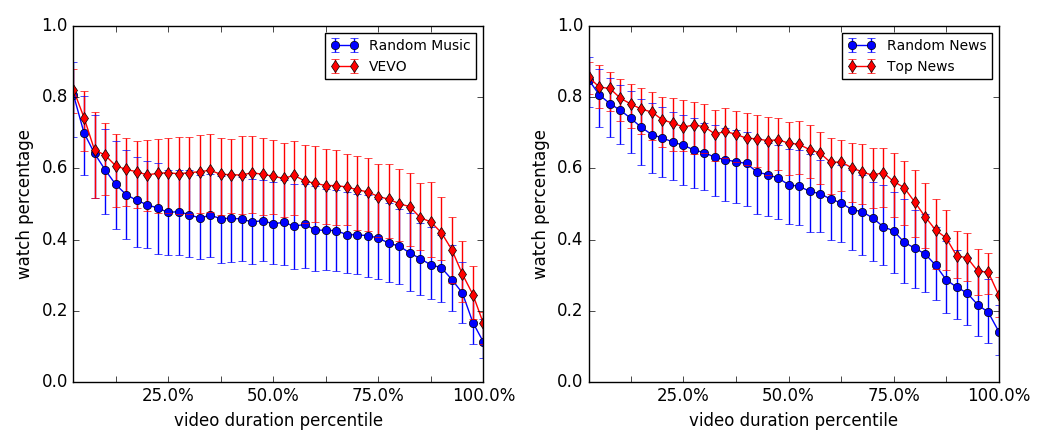
\includegraphics[scale=0.32]{external_source_comp.png}
    \caption{External Source Validation}
\end{figure}

Output: quality video dataset sit on top of random video dataset.


\subsection{Old videos and dedicated audience}

Hypotheses: when a video gets older, it will attract more dedicated audience thus appears as a growing watch percentage, even though views decrease.

Questions here: how to defind old? (moving truncated?) and how to express growth?

Note: fewer views inevitable result in larger variance of watch percentage.

Output: whether or not it hits dedicated audience?


%----------------------------------------------------------------------------------------

\section{Cold start watch behavior prediction}

\subsection{Classify Quality Videos}
How well can this model with a floating quality threshold?

input: a new video, with metadata only (video features, user vector)

output: is this a quality video? (appear above the top x\% of duration percentile plot)

method: classification task; category, duration as control variable.

setup: 

\subsection{Predict Watch Percentage}
input: a new video, with metadata only (video features, user vector)

output: what's the watch percentage by day 30? performance matrix to select features

method: regression task; category, duration as control variable.

setup: 

%----------------------------------------------------------------------------------------

\section{Integrate with HIP: Predict future watch time}
HIP model, learn a set of parameters to map dailyshare to dailywatch

Question: does this model work better with watch percentage plugged in?

input: a new video, with observed dailyshare, dailywatch, daily watch percentage

output: a line that fit video watch time in entire (120? 30?) lifecycle, explain the video quality.

method: HIP and modified HIP

%----------------------------------------------------------------------------------------
%	REFERENCE LIST
%----------------------------------------------------------------------------------------

\begin{thebibliography}{}

\bibitem[Park, Naaman and Berger 2016]{Park:2016data}
Park, M.; Naaman, M.; and Berger, J.
\newblock 2016.
\newblock A Data-Driven Study of View Duration on YouTube.
\newblock In \textit{Tenth International AAAI Conference on Web and Social Media}.

\bibitem[Martin et al. 2016]{martin2016exploring}
Martin, T.; Hofman, J.M.; Sharma, A.; Anderson, A.; and Watts, D.J.
\newblock 2016.
\newblock Exploring limits to prediction in complex social systems.
\newblock In \textit{Proceedings of the 25th International Conference on World Wide Web}.

\bibitem[Yu, Xie and Sanner 2015]{Yu:2015lifecyle}
Yu, H.; Xie, L.; and Sanner, S.
\newblock 2015.
\newblock The Lifecyle of a Youtube Video: Phases, Content and Popularity.
\newblock In \textit{ICWSM}.
 
\end{thebibliography}

%----------------------------------------------------------------------------------------

\end{document}
